\documentclass[9pt]{beamer}

%for russian text
\usepackage[utf8]{inputenc}
\usepackage[english,russian]{babel}

%for images
\usepackage{graphicx}
\graphicspath{ {./images/} }
\usepackage{wrapfig}

\begin{document}


\begin{frame} %17
\frametitle{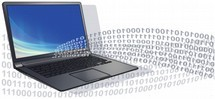
\includegraphics[width=2cm]{comp}\hfill М\textcolor{gray}{ера количества информации по Шеннону}\\ \hfill \noindent\rule{10.5cm}{0.4pt}}

\begin{wrapfigure}[7]{r}{0.2\textwidth}
\vspace*{-0.5cm}
\centering
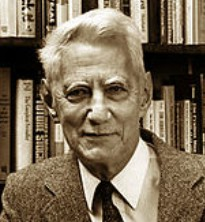
\includegraphics[width=2cm]{shennon}
\footnotesize Клод Шеннон(1916--2001)
\end{wrapfigure}

Мера Хартли подходит лишь для систем с равновероятными состояниями. Если состояния системы S не равновероятны, используют меру Шеннона:\\

\begin{centering}
$\displaystyle i(S) = -\sum_{i=1}^{N} p_{i}\cdot \log_{2} p_{i},$\\
\end{centering}

где $N$ – число состояний системы, $р_{i}$ – вероятность того, что система $S$ находится всостоянии $i$ (сумма всех $p_{i}$ равна 1).\\

\begin{centering}
\textbf{\textcolor{teal}{Формула Хартли является частным случаем формулы Шеннона!}}\\
\end{centering}

\textbf{Пример 1.} Количество информации в акте подбрасывания обычной монеты по формуле Хартли равно $\log_{2} 2 = 1$ бит. По формуле Шеннона получим то же: $i_{s1} = -0,5\cdot \log_{2} 0,5 - 0,5 \cdot \log_{2} 0,5 = 1$ бит.\\
\textbf{Пример 2.} При подбрасывании монеты со смещённым центром тяжести количество
непредсказуемости становится меньше: $i_{s2} = -0,75\cdot \log_{2}0,75 - 0,25\cdot \log_{2}0,25 \approx  0,8$ бит.
\end{frame}


\begin{frame} %18
\frametitle{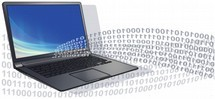
\includegraphics[width=2cm]{comp}\hfill П\textcolor{gray}{ример использования меры Шеннона}\\ \hfill \noindent\rule{10.5cm}{0.4pt}}
Шулер наугад вытаскивает одну карту из стопки, содержащей 9 известных ему карт: 3
джокера, 3 туза, 1 король, 1 дама и 1 валет. Какое количество информации для шулера
содержится в этом событии s?\\
\vspace*{1ex}
\begin{centering}
\begin{tabular}{ c c c c }
&джокера&&$3/9$ = $1/3$\\
&туза&&3/9 = 1/3\\
Вероятность вытащить\Huge\{&короля&\Huge\} \normalsize  равна& 1/9\\
&даму&&1/9\\
&валета&&1/9\\
\end{tabular}
\end{centering}
Количество информации, выраженное в тритах, равно:\\
$\displaystyle i(S) = - (\frac{1}{3}\cdot\log_{3}\frac{1}{3} + \frac{1}{3}\cdot\log_{3}\frac{1}{3}+ \frac{1}{9}\cdot\log_{3}\frac{1}{9}+\frac{1}{9}\cdot\log_{3}\frac{\bar{1}}{9}+\frac{1}{9}\cdot\log_{3}\frac{1}{9}) =$\\
$\displaystyle= \frac{1}{3} + \frac{1}{3} + \frac{2}{9} + \frac{2}{9} + \frac{2}{9} = 1\frac{1}{3} \approx \log_{3}5\hspace{1ex}vs\hspace{1ex} log_{3}14$
\end{frame}


\begin{frame} %19
\frametitle{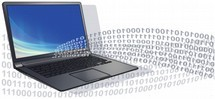
\includegraphics[width=2cm]{comp}\hfill Н\textcolor{gray}{естрогий вывод формулы Шеннона}\\ \hfill \noindent\rule{10.5cm}{0.4pt}}
\textbf{\textcolor{teal}{Задача.}} Монета имеет смещённый центр тяжести. Вероятность выпадения «орла» – 0,25,
вероятность выпадения «решки» – 0,75. Какое количество информации содержится в одном
подбрасывании?\\
\textbf{\textcolor{teal}{Решение}}\\
\begin{itemize}
\item Пусть монета была подброшена $N$ раз $(N\rightarrow \infty)$, из которых «решка» выпала $M$ раз, «орёл» — $K$ раз (очевидно, что $N = M + K$).
\item Количество информации в $N$ подбрасываниях: $i_{N} = M\cdot i$(«решка») $+ K\cdot i$(«орёл»).
\item Тогда среднее количество информации в одном подбрасывании: $i_{1} = i_{N}/N = (M/N)\cdot i$(«решка»)$+(K/N)\cdot i$(«орёл»)$ = p$(«решка»)$\cdot i$(«решка»)$+p$(«орёл»)$\cdot i$(«орёл»).
\item Подставив формулу Шеннона для $i$, окончательно получим: $i_{1} = -p$(«решка»)$\cdot \log_{x}p$(«решка»)$ - p$(«орёл»)$\cdot \log_{x}p$(«орёл»)$ \approx 0,8$ бит.
\end{itemize}
\end{frame}


\begin{frame} %20
\frametitle{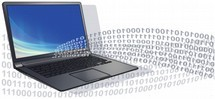
\includegraphics[width=2cm]{comp}\hfill П\textcolor{gray}{риставки для единиц измерения количества информации/данных: проблема}\\ \hfill \noindent\rule{10.5cm}{0.4pt}}

\begin{figure}[h]
\begin{minipage}{0.5\textwidth}
\centering
\caption{Linux Ubuntu 14}
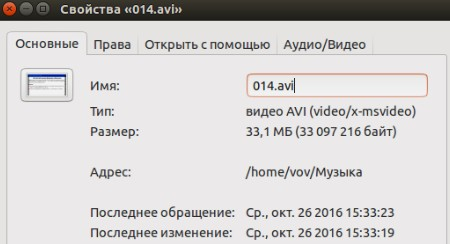
\includegraphics[width=.9\linewidth]{linuximg}
\end{minipage}\hfill
\begin{minipage}{0.5\textwidth}
\centering
\caption{Microsoft Windows 7}
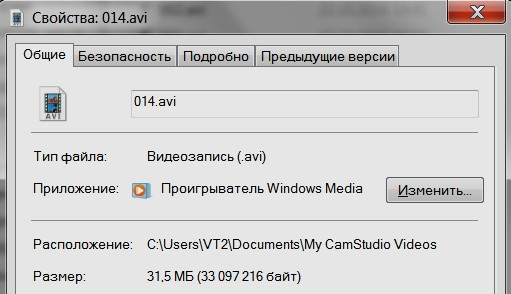
\includegraphics[width=.9\linewidth]{microsoftimg}
\end{minipage}
\end{figure}
\centering
33 097 216 байт — это \textbf{\textcolor{teal}{33,1}} МБ или \textbf{\textcolor{teal}{31,5}} МБ?

\end{frame}


\begin{frame} %21
\frametitle{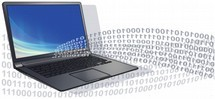
\includegraphics[width=2cm]{comp}\hfill П\textcolor{gray}{риставки для единиц измерения количества информации/данных: решение}\\ \hfill \noindent\rule{10.5cm}{0.4pt}}
\textbf{1. \textcolor{teal}{IEEE 1541-2002}} – Институт инженеров по электротехнике и радиоэлектронике.\\
\textbf{2. \textcolor{teal}{ISO/IEC 80000-13:2008}} – Международная организация по стандартизации.\\
\textbf{3. \textcolor{teal}{ГОСТ IEC 60027-2-2015}} – Международная электротехническая комиссия.\\

\begin{centering}
\begin{tabular}{ |c |c| c| }
\hline
Приставки единиц СИ&Новые двоичные префиксы&$\Delta,\%$\\
\hline
килобайт (kB) $= 10^{3}$ байт&кибибайт (KiB, КиБ) $= 2^{10}$ байт&2\\
\hline
мегабайт (MB) $= 10^{6}$ байт&мебибайт (MiB, МиБ) $= 2^{20}$ байт&5\\
\hline
гигабайт (GB) $= 10^{9}$ байт&гибибайт (GiB, ГиБ) $= 2^{30}$ байт&7\\
\hline
терабайт (TB) $= 10^{12}$ байт&тебибайт (TiB, ТиБ) $= 2^{40}$ байт&10\\
\hline
\end{tabular}
\end{centering}

\textbf{\textcolor{teal}{Краткое обозначение битов и байтов}}: b = bit = бит, B = Б = байт\\
1024 B = 1024 Б = 8192 b = 8192 бит = 8 Кибит = 1 КиБ = 1 KiB
\end{frame}


\end{document}